\documentclass[12pt]{article}
\usepackage{fullpage}
\usepackage{graphicx, rotating, booktabs} 
\usepackage{times} 
\usepackage{fbb} 
\usepackage{natbib} 
\usepackage{indentfirst} 
\usepackage{setspace}
\usepackage{grffile} 
\usepackage{hyperref}
\usepackage{tikz-cd}
 \usetikzlibrary{cd}
\usepackage[export]{adjustbox}
\usepackage[most]{tcolorbox}
\usepackage{verbatimbox}
\usepackage{lscape}
\usepackage{afterpage}
\usepackage{amsmath}
\usepackage[labelfont={bf},textfont=it,labelsep=period]{caption}
 \usepackage{multirow} 
\setcitestyle{aysep{}}
\usepackage{dcolumn}

\hypersetup{
  colorlinks = true,
  urlcolor = blue,
  linkcolor = black,
  citecolor = black,
  pdfauthor = {Joshua Alley},
  pdfkeywords = {},
  pdftitle = {},
  pdfsubject = {},
  pdfpagemode = UseNone,
%  pdffitwindow = true
%  pdfcenterwindow = true
}



\singlespace
\title{\textbf{Using Bayesian Hierarchical Models to Estimate Heterogeneous Effects}}
\author{Joshua Alley \\
Assistant Professor \\
University College Dublin\thanks{Thanks to Carlisle Rainey for helpful comments.} \\
joshua.alley@ucd.ie
}

 
\date{\today}

\bibliographystyle{apsr}

\usepackage{sectsty}
\sectionfont{\Large}
\subsectionfont{\noindent\large\textit}
\subsubsectionfont{\normalsize}

\makeatletter
\renewcommand\tiny{\@setfontsize\tiny{9}{10}}
\makeatother


\begin{document}

\maketitle 

\begin{abstract} 
Heterogeneous effects are common in social science. 
In this note, I introduce a Bayesian hierarchical approach to estimating heterogeneous effects. 
The modeling strategy uses varying slopes and intercepts, along with predictors of the slopes, to capture heterogeneous effects by groups.  
Researchers can use the results to infer how different factors modify an effect and how groups with unique combinations of those factors respond to an independent variable. 
This approach provides an intermediate tool between interactions or subgroup analyses and machine-learning approaches for discovering complex heterogeneity. 
It is more flexible than interactions and reduces the risk of underpowered subgroup comparisons.
At the same time, it is more theoretically driven and interpretable than some machine-learning approaches, as well as easier to implement in small datasets. 
Researchers can thus use hierarchical models alongside other approaches to understand heterogeneous effects for scholarship and policy.
\end{abstract} 


\newpage 
\doublespace 


\section{Introduction}


% one: het effects matter
Whether in observational and experimental studies, every independent variable social scientists study impacts some units more or less than others. 
Aggregate relationships often mask heterogeneous effects.\footnote{\citet{Abramsonetal2022} note that the average marginal component effect (AMCE) of conjoint experiments reflects the direction and intensity of respondent preferences, and gives more weight to intense preferences.} 
In some circumstances, these averages are useful, but in many cases, they mask interesting and important variation. 


As a result, understanding varying responses to the same stimulus is essential for policy and scholarship. 
Scholars can better elucidate the process linking their independent variable and outcome.
Policymakers can target finite resources. 


% expand/sharpen this 

% two: introduce my solution 
This note introduces a hierarchical Bayesian approach to estimating heterogeneous effects. 
The technique uses varying slopes and intercepts, along with covariates, to estimate heterogeneous effects. 
Modeling heterogeneous effects in this way is produces easily interpretable results, which facilitates argument testing. 
It also allows researchers to compare different sources of heterogeneous effects, and can be extended in many ways.  
Implementation using the brms package for \textsf{R} is straightforward.\footnote{Researchers can also calculate marginal effects by group easily with the marginaleffects package \citep{ArelBundockme}}. 


% three: loads of techniques
This approach to heterogeneous effects fills a niche between existing tools for estimating heterogeneous effects.
Parametric interactions and subgroup analyses are a common way that scholars examine individual modifiers. 
While these techniques are easy to implement and interpret, they lose their ease of interpretation with more than three dimensions and are often misleadingly underpowered \citep{Simmonsetal2011}.\footnote{\citet{BlackwellOlson2022} describe a lasso approach to interactions that is also an intermediate step between machine-learning and linear regressions.}
To capture more complex variation, later recent work employs random forests \citep{GreenKern2012, WagerAthey2018}, support vector machines \citep{ImaiRatkovic2013}, and ensemble methods \citep{Grimmeretal2017, Kuenzeletal2019, Dorieetal2022}.
These machine learning algorithms capture complex patterns, but can be harder to interpret and implement, especially in smaller datasets. 

 
 
Using a hierarchical model where other variables predict heterogeneous effects is more flexible than simple parametric interactions but easier to employ than machine learning approaches.  
It preserves a simple and interpretable structure like interactions, while accommodating more factors and reducing the risks of subgroup analysis. 
This facilitates argument testing and is easier to interpret than some machine-learning techniques.
The hierarchical approach lacks the flexibility to discover high-dimensional heterogeneity, however.  
As a result, this approach is best used in concert with other heterogeneous effects techniques, and could be a useful addition to ensemble models. 


% wrap and introduce the application 
In the remainder of this note, I describe the model and demonstrate how it works by analyzing a study of how foreign side-taking in US elections impacts support for economic engagement by \citet{BushPrather2020}.  
While substantiating the original findings, the reanalysis also reveals that gender and political engagement shape how foreign side-taking in elections impacts support for economic engagement.



\section{A Hierarchical Model of Heterogeneous Effects}


The heterogeneous effects model uses at least two equations, and is easiest to estimate with Bayesian methods.\footnote{Priors for most parameters depend on the problem and researcher knowledge. I estimate the example model below with STAN \citep{Carpenteretal2016}.} 
The first equation links the treatment and outcome. 
The second equation estimates heterogeneous effects as a function of unit characteristics, other treatments, contextual factors, or whatever else the researcher is interested in. 
The estimates give heterogeneous effects for groups with unique combinations of variables that modify the treatment and correlates of differences in the treatment.\footnote{Adding additional heterogeneous effect equations to estimate heterogeneous effects for multiple variables is straightforward.}  


This approach can apply to many problems, but the following example addresses a common scenario; making between-unit comparisons based on an experimental treatment.    
Start with \textit{N} units indexed by \textit{i}, some of which receive a binary treatment \textit{T}.
For simplicity, I assume that the outcome variable ${y}$ is normally distributed with mean $\mu_i$ and standard deviation $\sigma$.\footnote{Researchers should use binary, categorical and other outcome likelihoods as needed.}


The first equation predicts the outcome mean. 
The outcome for each unit is then a function of varying intercepts $\alpha_g$, a matrix of control variables \textbf{X},\footnote{This can be omitted, depending on the application. Adding additional grouping structures for more complex data is also straightforward.} and a set of group treatment effects $\theta_g$, which are normally distributed with mean $\eta_g$ and standard deviation $\sigma_\theta$. 
The researcher divides all units into \textit{g} groups based on unique combinations predictors of heterogeneous effects \textbf{Z}. 
Each $\theta$ parameter estimates the treatment effect in group \textit{g}, and is often referred to as a varying slope. 


\begin{equation}
\begin{aligned}
y &\sim N(\mu_i, \sigma) &\text{(Likelihood)} \\
\mu_i &= \alpha_g + \theta_g \textit{T} + \textbf{X} \beta &\text{(Mean Equation)}  \\
\theta_g &\sim N(\eta_g, \sigma_\theta) \\ 
\eta_g &= \lambda_g + \textbf{Z} \lambda &\text{(Heterogeneous Effects)} 
\end{aligned}
\end{equation}


The second equation then predicts the treatment effects with a second set of variables in the matrix \textbf{Z}. 
\textbf{Z} can contain anything that modifies the impact of treatment, including unit characteristics, other treatments, or contextual factors. 
The researcher specifies these variables and uses them to define the groups. 
The second equation also includes an intercept $\lambda_g$ that estimates the impact of treatment when all the heterogeneous effect variables are zero.
As in other regressions, this intercept is not always substantively meaningful.\footnote{In most applications, the random intercepts $\alpha_g$ and varying slopes $theta_g$ should have a common multivariate normal prior to capture correlations between group slopes and intercepts.}


% Interpretation 
The $\theta$ parameters are the key estimates in this model.
These give the impact of a treatment within each group as a function of a systematic component where the group-level variables in \textbf{Z} modify the varying slope directly, and a random component. 
The impact of a treatment within groups is also correlated with the group mean $\alpha_g$.  


% a word on groups 
Specifying the groups in which treatment slopes vary is the most important task for researchers. 
Setting groups determines how treatment slopes vary.
As in almost every social science application, researchers should identify what variation is most important and interesting. 
This requires theoretical or policy guidance. 


% three ways to set groups
There are three general ways to set groups.
First, if an intervention has multiple dimensions, researchers might set groups using combinations of other treatments.
This uses the hierarchical model to estimate heterogeneous treatments and the experimental design determines groups. 
A second approach uses unit and contextual factors to create groups and estimate treatment effect heterogeneity. 
In this instance, researchers examine what within or around units shapes their reaction to an intervention.\footnote{For example, \citet{Alley2021isq} uses alliance characteristics such as treaty design and membership to examine when alliance membership increases or decreases military spending.} 
Third, researchers may have specific policy aims, for example if they want to understand how an intervention affects individuals in a specific population in a given geography. 


% grouping factors: numbers 
The number of grouping factors will depend on a researcher's theoretical interest, but there may be some practical constraints. 
Dividing groups based on many factors will create many small groups and increase the risk of model convergence problems. 
Using only one factor will create an unidentified model, and researchers should use interactions in this case. 


% advantages 
Estimating heterogeneous effects in this way has three advantages.
First, this model allows researchers to account for multiple potential sources of heterogeneous effects in an easy to interpret framework. 
Researchers can thus examine theories of heterogeneous effects and compare sources of variation.\footnote{Rescaling variables in the heterogeneous effects equation, for example by rescaling continuous variables by two standard deviations \citep{Gelman2008}, can aid model fitting and direct coefficient comparisons.} 
Partial pooling also facilitates reasonable estimates for small groups by sharing information across treated groups and leveraging the predictors in the heterogeneous effects equation. 
Finally, this approach will be faster than machine learning approaches for many datasets, and may scale better than models that attempt to estimate individual treatment effects.


% disadvantages
Like all methods, this technique has downsides, which can be partially ameliorated by altering the basic framework above. 
Because groups are based on unique combinations of heterogeneous effect variables, using multiple continuous variables in the heterogeneous effects equation creates many small groups or individual treatment effects, which increases the risk of sampling problems, especially in small datasets. 
If using several continuous variables hinders model convergence, researchers can bin continuous variables.


Furthermore, unlike machine learning approaches, this model will not discover high-dimensional interactions. 
That said, researchers can inject substantial flexibility if they want using additional interactions or non-linear specifications in either level of the model. 
Third, this model can show general trends, but will not make powerful comparisons between every groups. 
Researchers who want to compare a few specific groups may not be able to, especially if the groups are small.



\section{Example Application} 


In the following, I demonstrate how the model works by reanalyzing a study by \citet{BushPrather2020} (BP hereafter). 
This study examines how foreign meddling in elections impacts support for economic engagement with the meddler. 
One of their experiments examines how Russian or German engagement in the 2016 US election impacts mass support for trade and investment with those countries.
I use a heterogeneous effects model to check their results and further explore their findings. 


% describe design
BP employ a 2x2x2 factorial experiment.
This design randomizes whether a foreign country is interfering in the 2016 election, the country and their attitude towards Trump and whether the potential economic ties entail greater trade or investment in the United States.
In one treatment, Russia expresses support for Trump and in the other, Germany expresses opposition to Trump. 


BP hypothesize that individuals will prefer economic engagement with states that support their candidate. 
They thus examine how the impact of side-taking varies with the direction of the endorsement, individual political preferences, and the economic issue. 
To do this, they use four tables and figures, and rely on eight t-tests of differences in means between groups of roughly 25 respondents. 


The heterogeneous effects model encapsulates the argument and all tests by estimating the impact of side-taking on economic engagement as a function of which country is involved, a dummy indicator of intention to vote for Clinton, and their interaction. 
The interaction captures the hypothesis that Clinton voters will support engagement with Germany because Germany opposed Trump, and should be positive. 
I also add an indicator of whether the experiment deals with trade or investment. 
Last the heterogeneous effects equation also includes indicators of female gender, active employment, college education, political knowledge, and political interest. 



The outcome variable is a scale from one to four that measures support for greater economic engagement with the potential partner. 
To approximate BP's analyses, I use a normal outcome likelihood. 
Because this experimental randomization produced a roughly balanced sample, I do not include any control variables in the outcome equation. 


\begin{figure}[htpb]
	\centering
		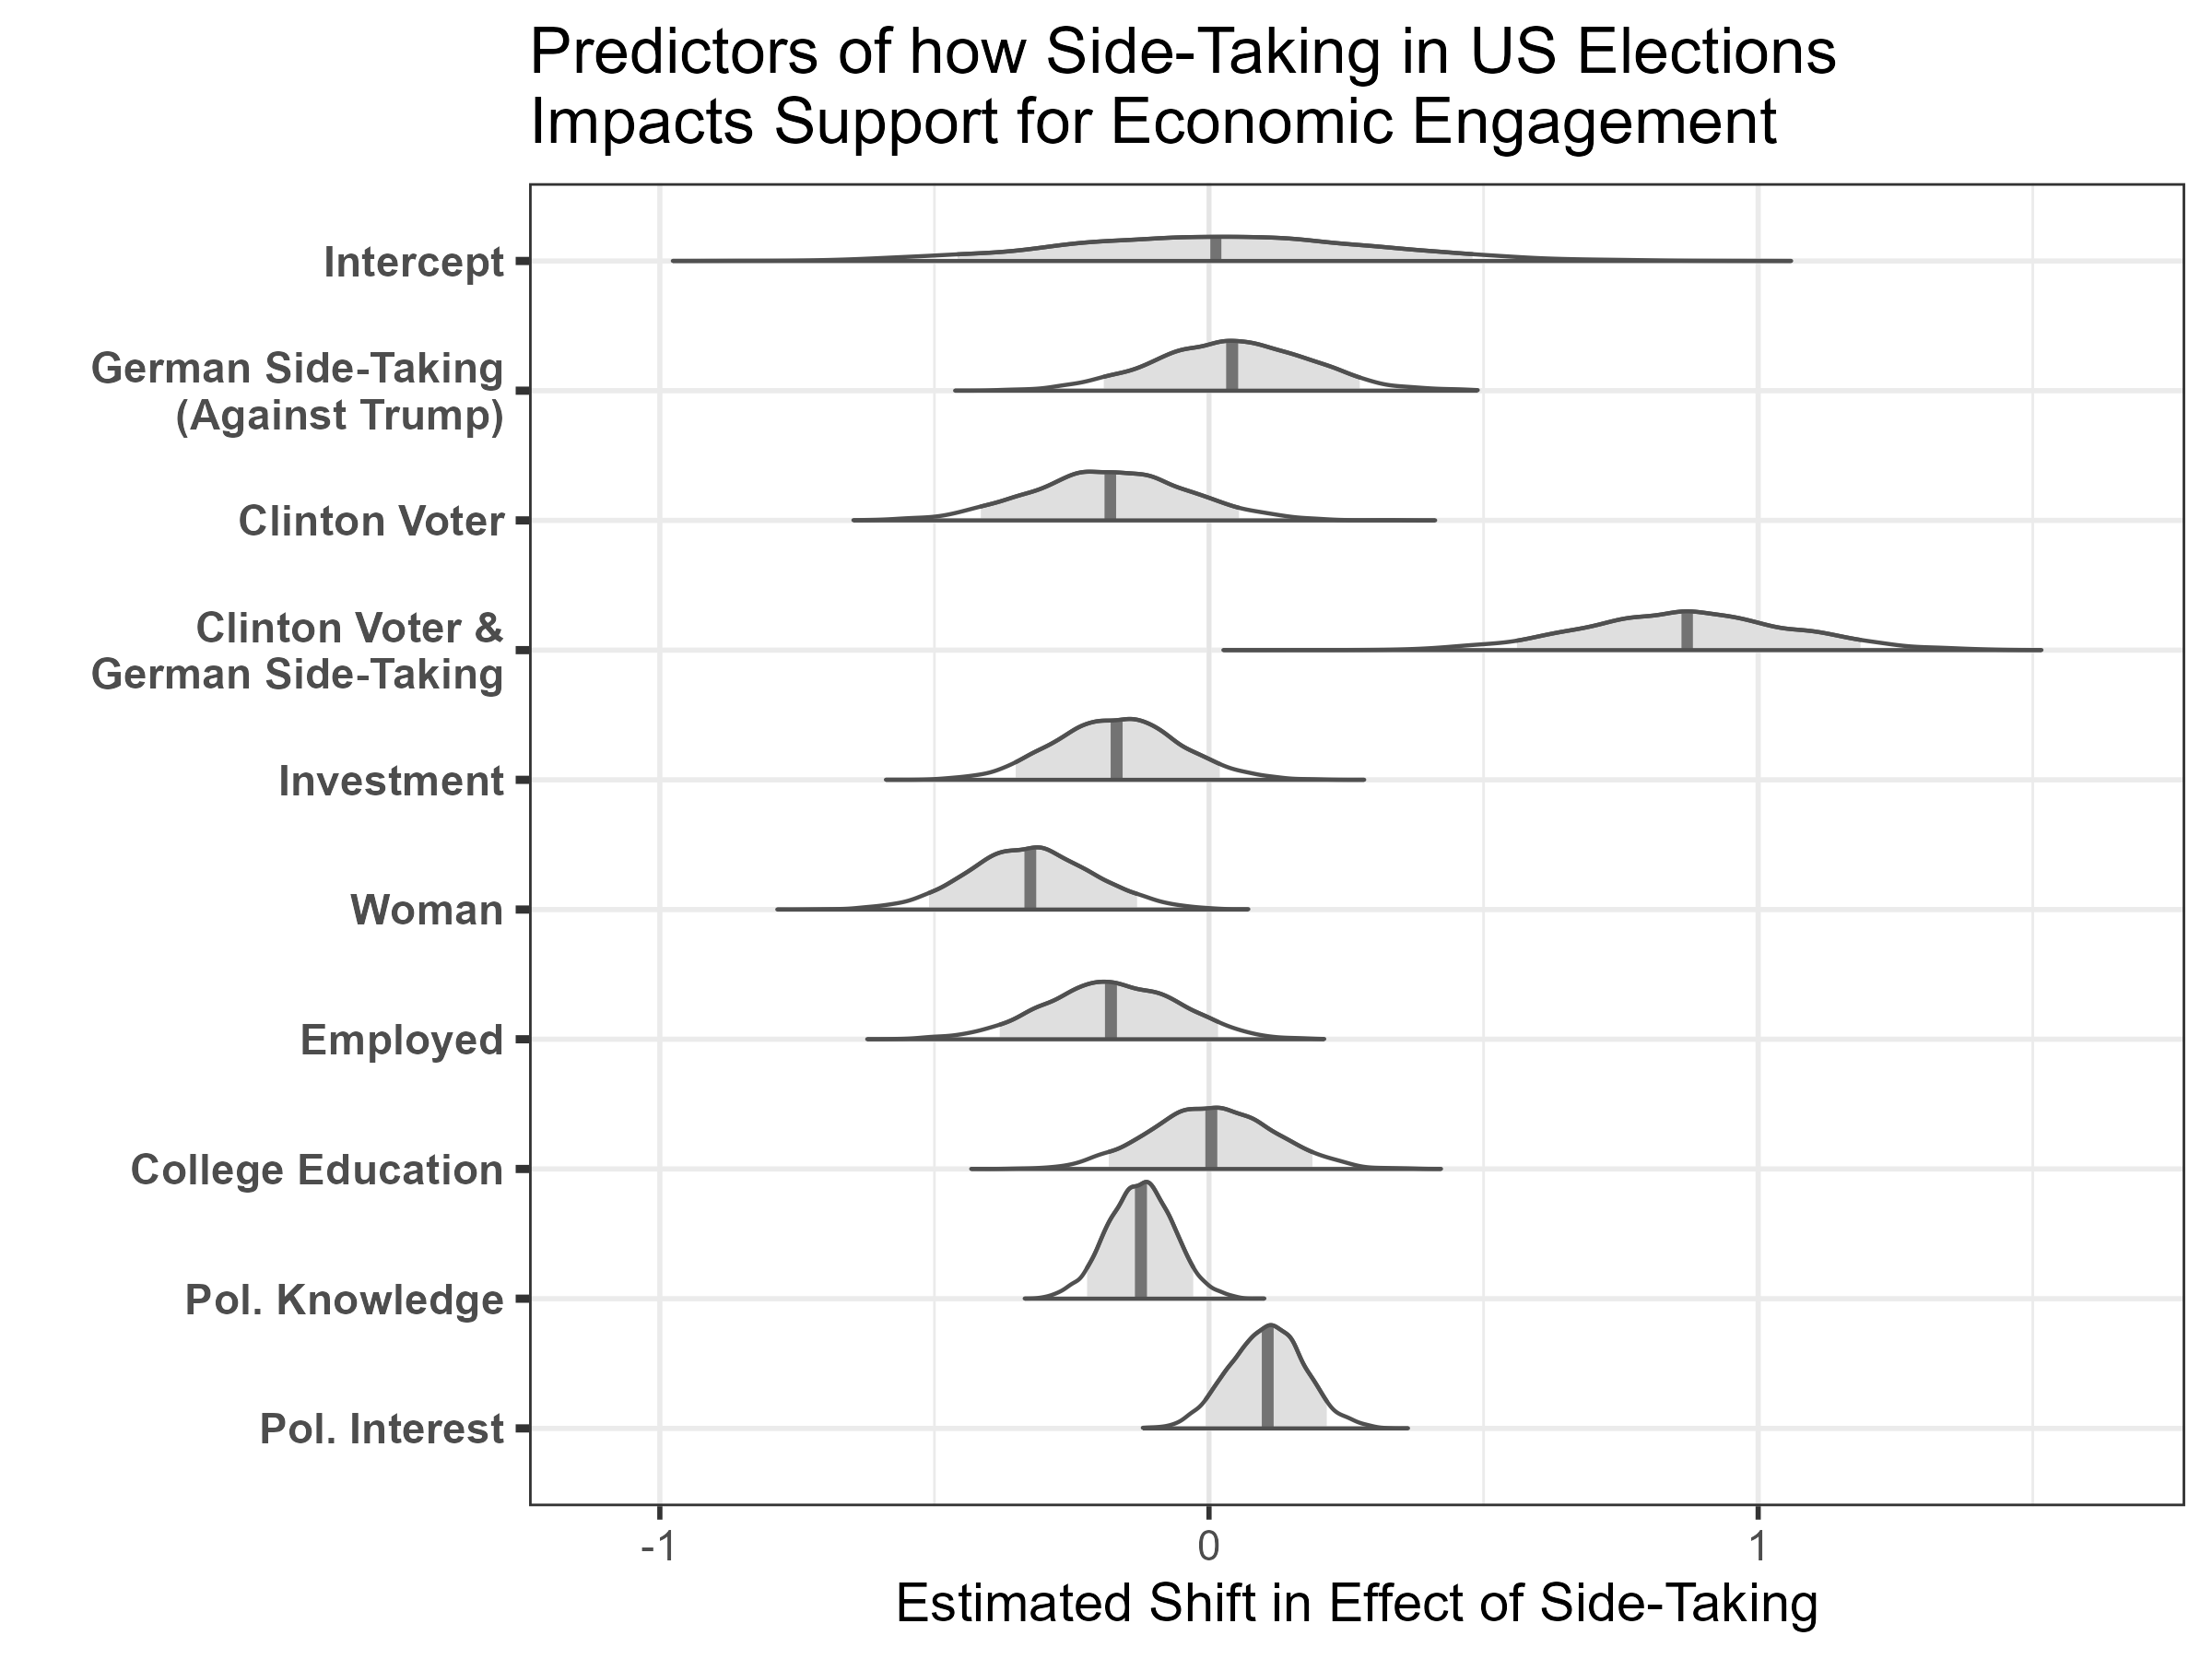
\includegraphics[width=0.95\textwidth]{../figures/bp-lambda.png}
	\caption{}
	\label{fig:bp-lambda}
\end{figure}


\autoref{fig:bp-lambda} summarizes the estimates from the heterogeneous effects equation. 
As BP predicted and find, side-taking increases support for economic engagement with voters whose candidate the intervention supports. 
Relative to the impact of Russian side-taking on Trump voters, German side-taking increases the impact of side taking by almost 1, which is a large difference on an outcome that ranges from 1 to 4. 
German side-taking does not impact Trump voter support for economic engagement, and Clinton voters are marginally but not clearly less supportive of engagement with Russia after Russian side-taking.
These estimates are consistent with BP's results. 


\begin{figure}[htpb]
	\centering
		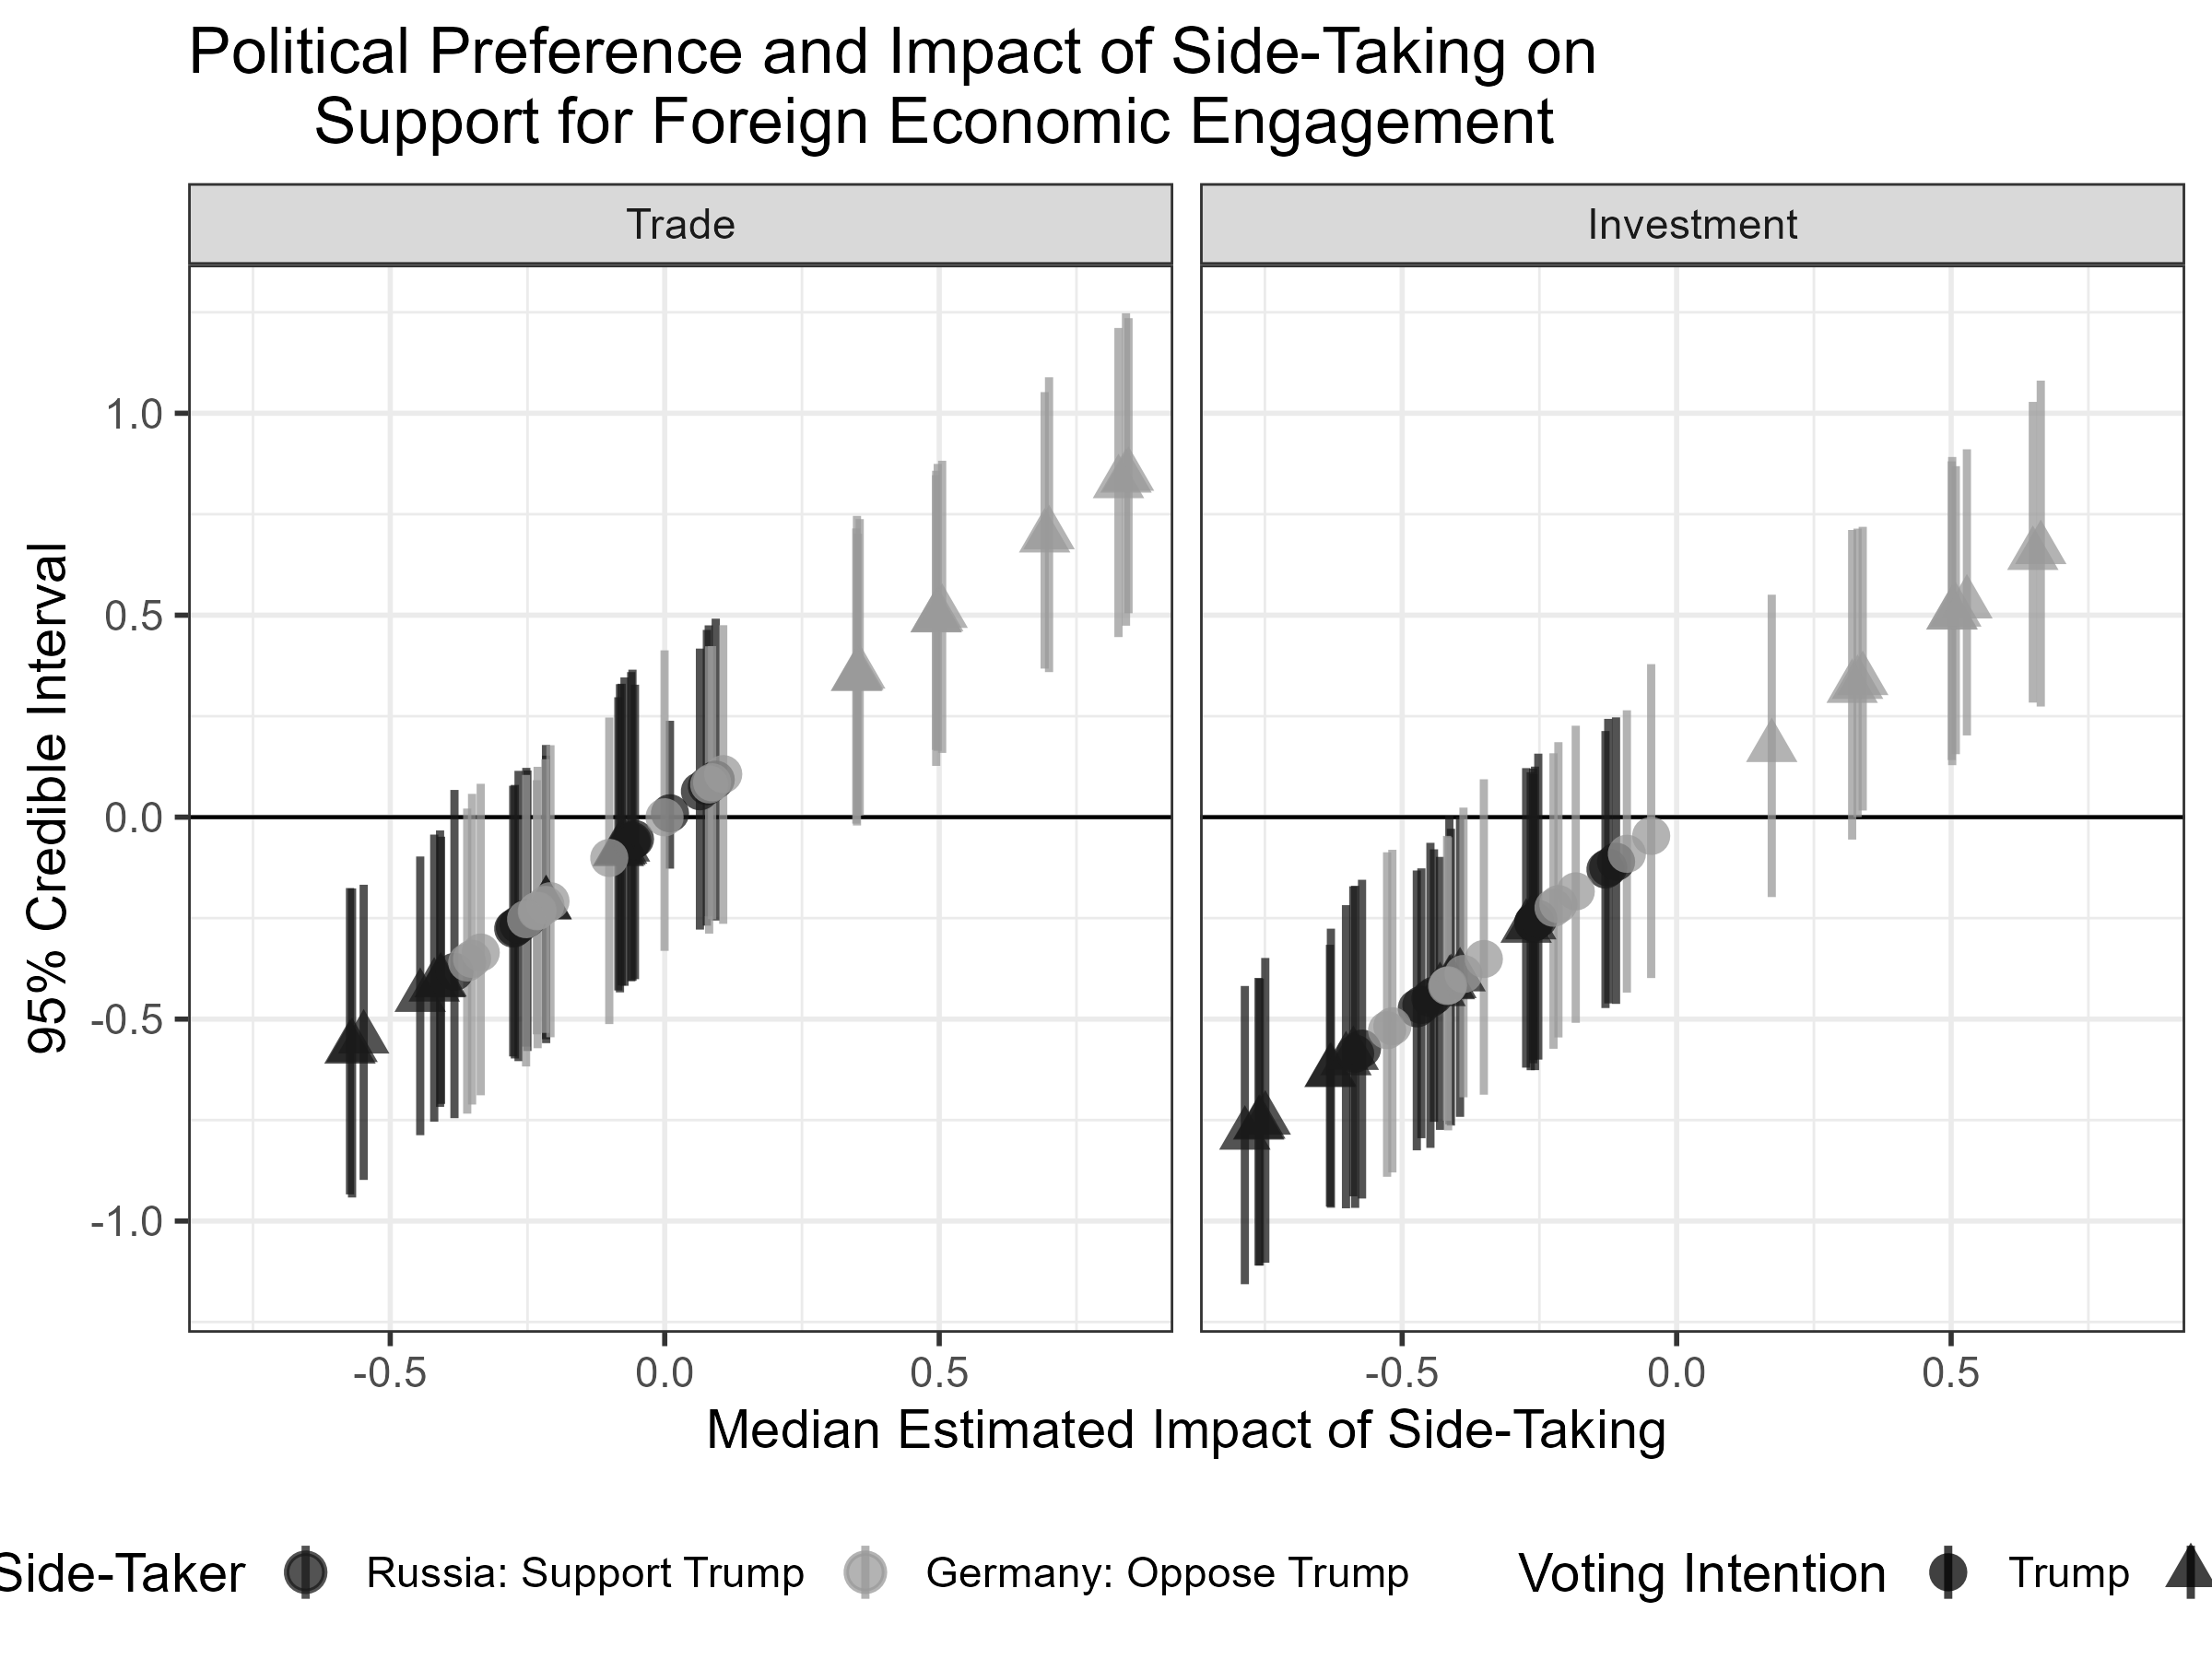
\includegraphics[width=0.95\textwidth]{../figures/bp-theta-est.png}
	\caption{Heterogeneous effects of foreign side-taking in US elections on support for economic engagement with the interfering country. Each estimate reflects a treated group with a unique combination of other treatments and demographic characteristics.}
	\label{fig:bp-theta-est}
\end{figure}


The model also provides some new information about how side-taking impacts support for economic engagement. 
Electoral side-taking is more likely to reduce support for foreign investment in the United States, all else equal. 
Moreover, women largely respond more negatively to side-taking. 
Finally, increasing political knowledge decreases the the impact of side-taking, while interest in politics increases it. 


\autoref{fig:bp-theta-est} substantiates these inferences and presents the group-specific treatment effects. 
In general, Clinton voters were more responsive to side-taking. 
Most Clinton voters were less likely to support trade and investment with Russia after exposure to Russian support for Trump, and more likely to back economic cooperation with Germany in response to German opposition to Trump. 
Additional variation in this relationship comes from gender and political engagement.
Some Trump voters reduce their support for investment regardless of who the intervention backs and are less likely to change their trade attitudes in response to side-taking as well. 


% power point
The credible intervals on these estimates suggest that researchers should not rely on this technique to generate powerful tests between groups, unless predictors of heterogeneous effects create substantial differences. 
For instance, most Trump voters hold very similar views of economic engagement, and there are only a few that are clearly different. 
Among Clinton voters, however, the response to German side-taking and corresponding distaste for Russian side-taking creates huge differences between different treated groups. 


\section{Conclusion}

This note introduced a simple and interpretable hierarchical technique for estimating heterogeneous effects. 
The approach above can apply to a wide range of outcomes, data structures, and theories. 
Explicitly modeling how different groups respond to an independent variable can help test new arguments and identify who responds best to a given intervention. 


Again, this approach is a complement for existing tools, not a substitute. 
Hierarchical modeling provides an intermediate approach between simple interactions or subgroup analyses and complex machine-learning algorithms. 
Researchers can thus use this tool to check other results or inform those techniques.
With this and other tools, scholars and policymakers can better understand heterogeneous effects.


\singlespace
 
\bibliography{../../MasterBibliography} 


\end{document}
